\section{Task 1}\label{sec:task1}
\graphicspath{ {./figures/} }

In this project we use the sructural ensamble PED00020 (measles virus nucleoprotein) with five models.
The goal of the first task is to implement a software to identify conformational relationships within a single ensemble.  The input of this task is a file containing the PDB structure of one single PED model.


\subsection{Single conformation features}
Relationships within an ensemble will be identified considering the structural features of single conformations.

First, the software extracts the single conformation features and it puts them into a unique dictionary for each model:
\begin{itemize}
\item Radius of gyration of the structure: it is computed using the coordinates of each atom and their barycenter.
\item Relative accessible surface area (ASA) for each residue: it should be noted that for within a conformation the ASA is the same.
\item Secondary structure for each residue: it computes the angles Phi and Psi and then get SS from them and compare with DSSP.
\item Residue distance matrix: it computes the pairwise distances between residues.
\end{itemize}

We have noticed that some conformations have a different number of residues. So we preprocessed each structure and added a zeros padding at the end if necessary.

\subsection{Representative conformations} 
In order to extract the representative conformations for each conformation, the software clusters all the models within a single ped using KMedoids methods and a customed metric function. 
We use KMedoids because can be used with arbitrary dissimilarity measures and minimizes a sum of pairwise dissimilarities. 
Furthermore, we use a specific metric function built using the calculated features and different types of distances to measure their distances. The function takes in input two residues and compute their distance that is a sum of the partial features distances.
The partial metrics are: 
\begin{itemize}
\item Absolute difference between radius of gyration.
\item Euclidian distance of ASA vectors.
\item Hamming distance between SS vectors beacause they are chars.
\item The complementary of correlation between distance matrix. 
\end{itemize}

Then the software compute the distance among the representative conformations by the same metric function and plot a weighted graph. The length of the edges is proportional to the distance between the two conformations in the nodes. The label in each node is the ID of the conformations.

\begin{figure}[H]
	\begin{minipage}[b]{0.47\textwidth}
		\centering
		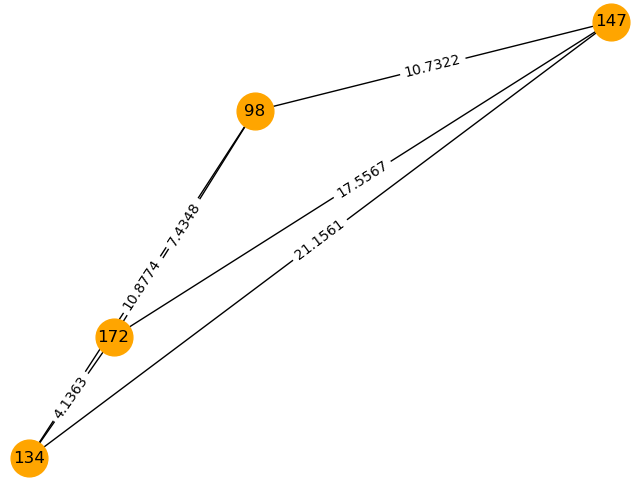
\includegraphics[width=\textwidth]{PED00020e001_graph.png}
		\caption{Graph of model 001.}
		\label{model001}
	\end{minipage}
	\hfill
	\begin{minipage}[b]{0.47\textwidth}
		\centering
		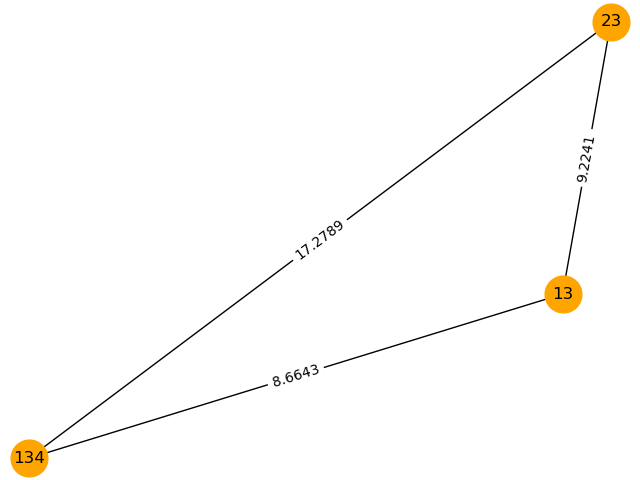
\includegraphics[width=\textwidth]{PED00020e002_graph.png}
		\caption{Graph of model 002.}
		\label{model002}
	\end{minipage}
	\hfill
	\begin{minipage}[b]{0.47\textwidth}
		\centering
		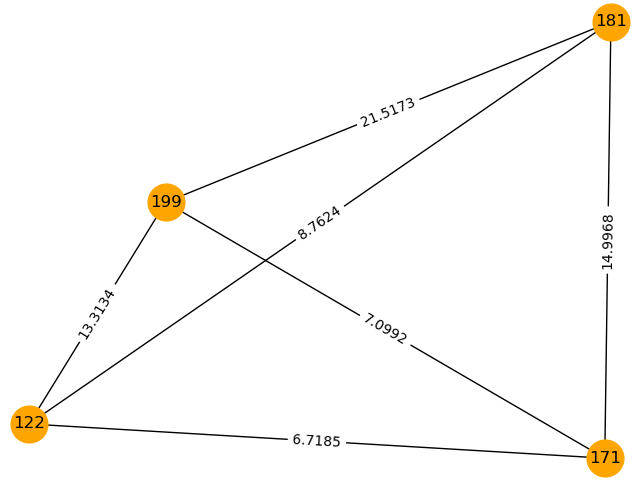
\includegraphics[width=\textwidth]{PED00020e003_graph.png}
		\caption{Graph of model 003.}
		\label{model003}
	\end{minipage}
	\begin{minipage}[b]{0.47\textwidth}
		\centering
		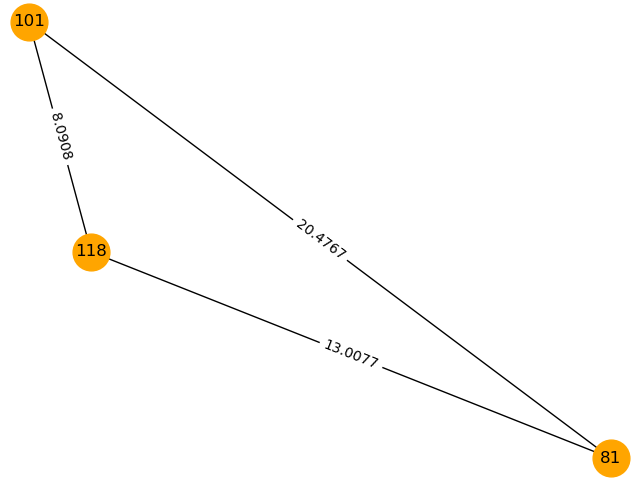
\includegraphics[width=\textwidth]{PED00020e004_graph.png}
		\caption{Graph of model 004.}
		\label{model004}
	\end{minipage}
	\hfill
	\begin{minipage}[b]{0.47\textwidth}
		\centering
		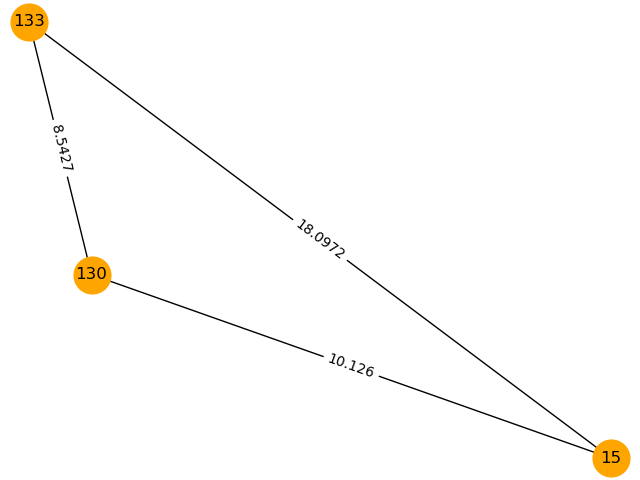
\includegraphics[width=\textwidth]{PED00020e005_graph.png}
		\caption{Graph of model 005.}
		\label{model005}
	\end{minipage}
	\end{figure}

By running the script several times, a high variability can be observed in the centroids found.
This is probably caused by the proximity of the points and the random initialization of clustering. The centroids will be different but with the same cardinality.
%
It can be observed that in the various ensemble, the distance between the centroids is different but the number of representative conformations is always the same.
%


\subsection{Pymol image}
For each ensemble, the software generates a pymol image to visualize the structure and through the variability of the colors, the distance between the residues of its representative conformations.

The color of the structure varies based on the distance between the residuals calculated using a metric built by us. This metric evaluates the variability of the features extracted for each position of the representative conformation. In the metric the radius of gyration is not used because it is constant.

We decided to generate different images for each ensemble because generating a superimposition of all the representative conformations extracted within the clustering step was insignificant and too messy.

\begin{figure}[H]
	\begin{minipage}[b]{0.47\textwidth}
		\centering
		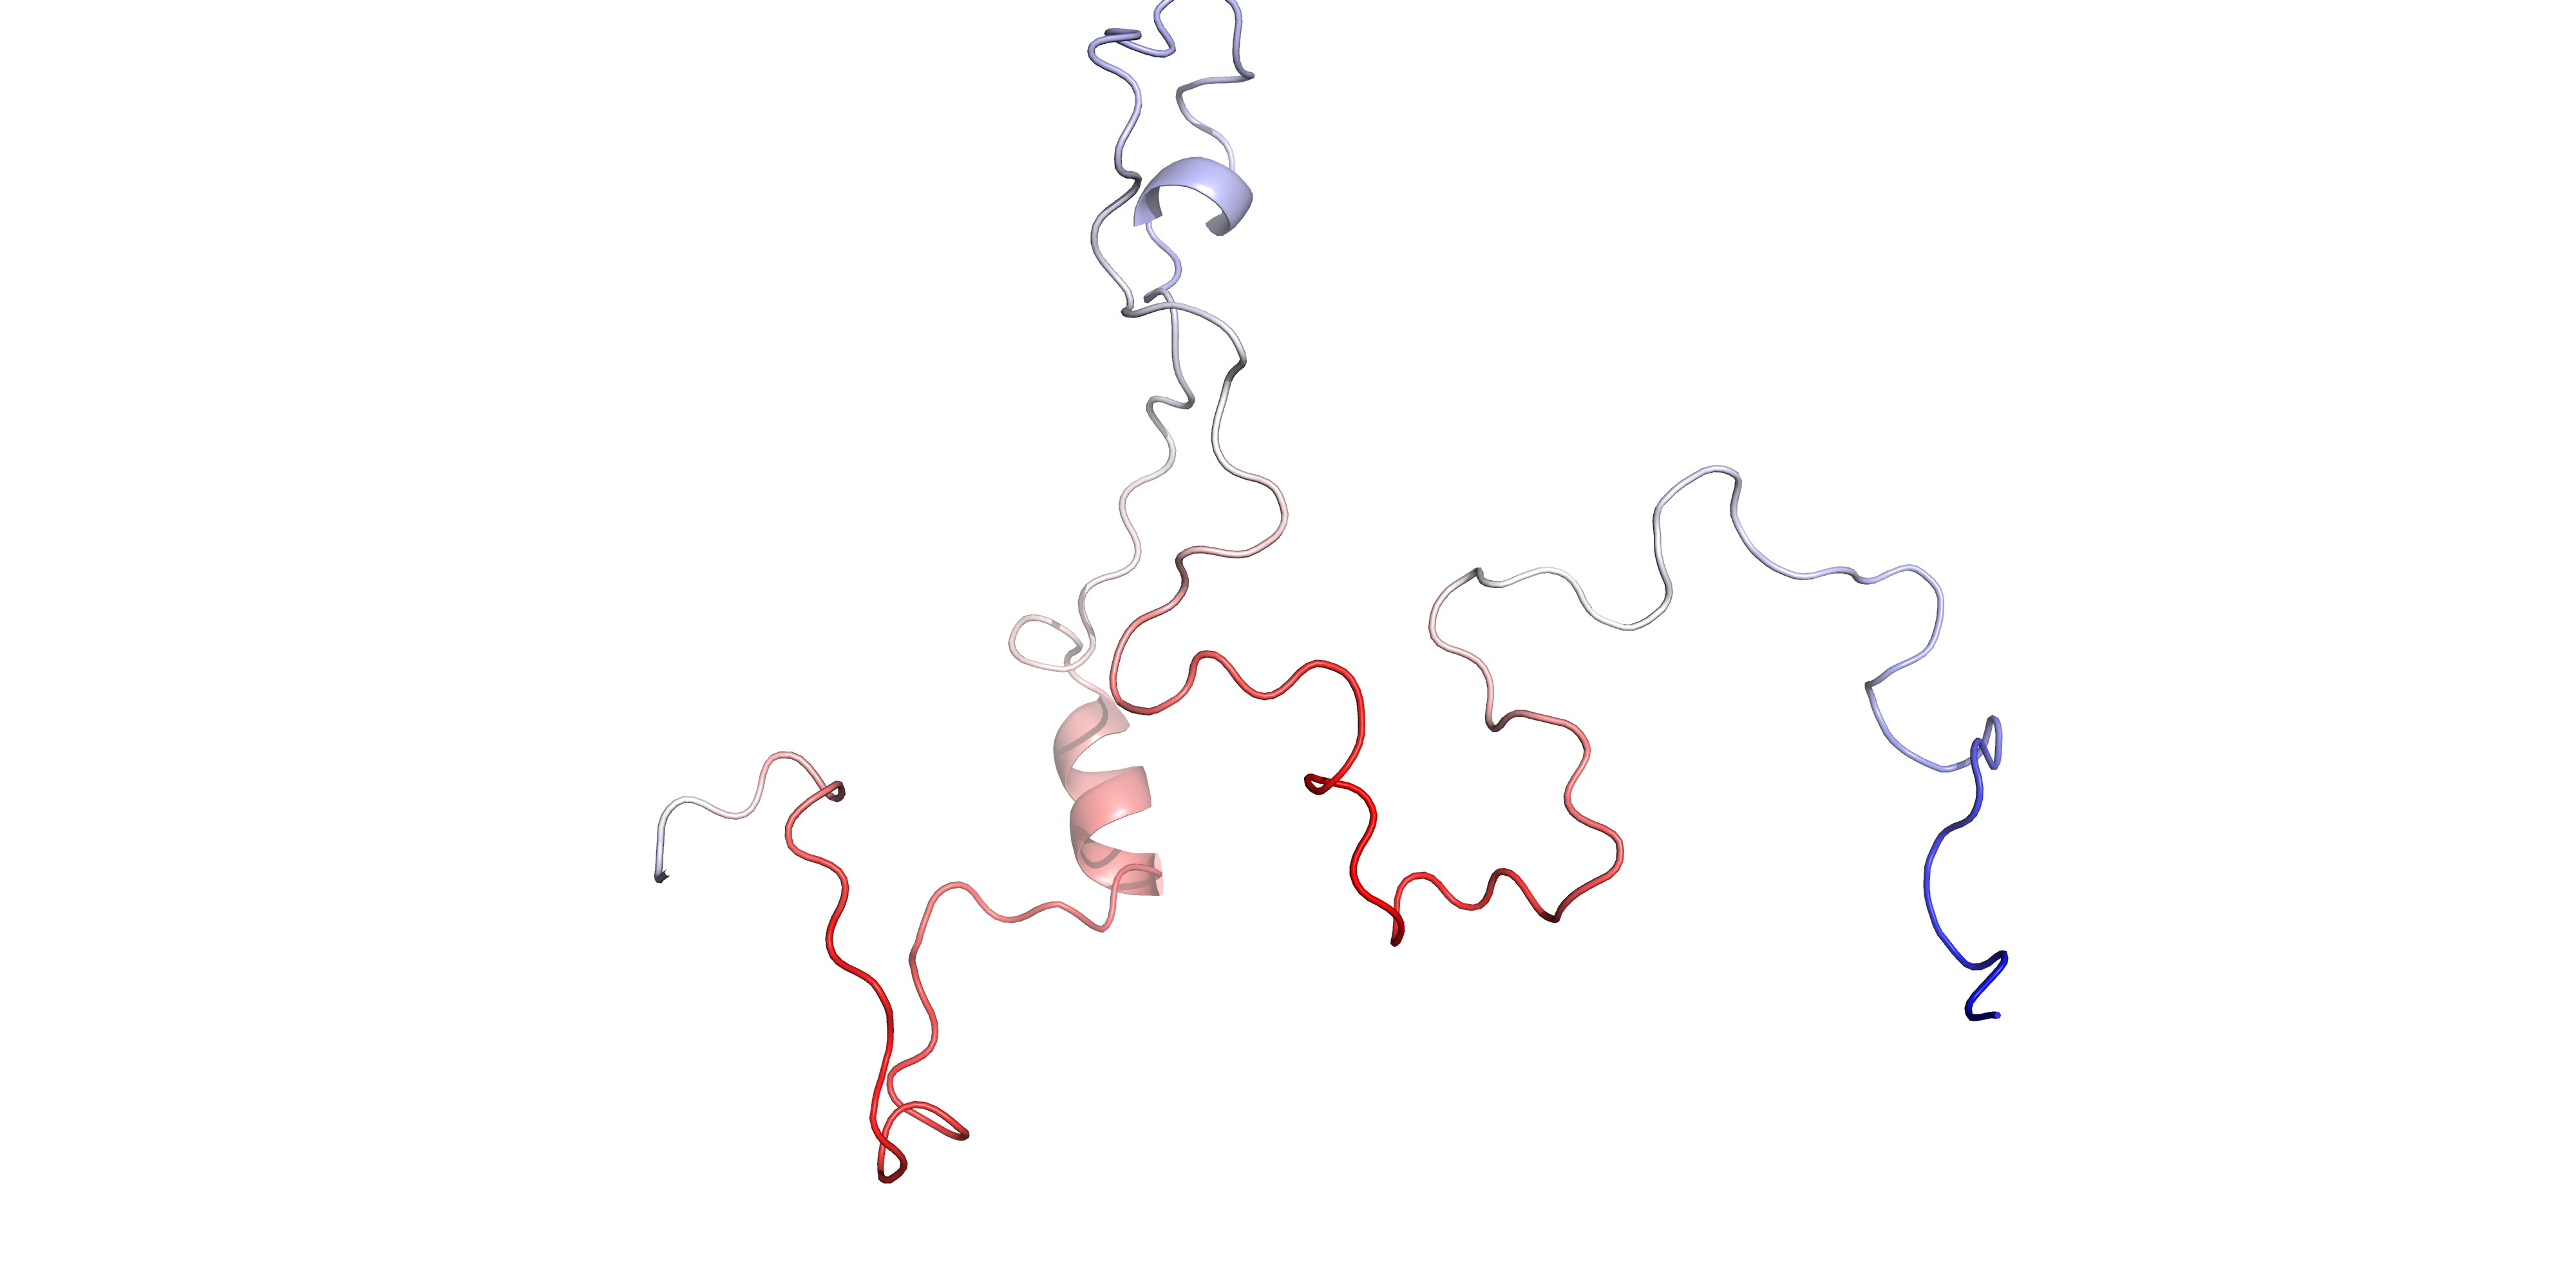
\includegraphics[width=\textwidth]{PED00020e001_pymol.png}
		\caption{Pymol image of model 001.}
		\label{model001}
	\end{minipage}
	\hfill
	\begin{minipage}[b]{0.47\textwidth}
		\centering
		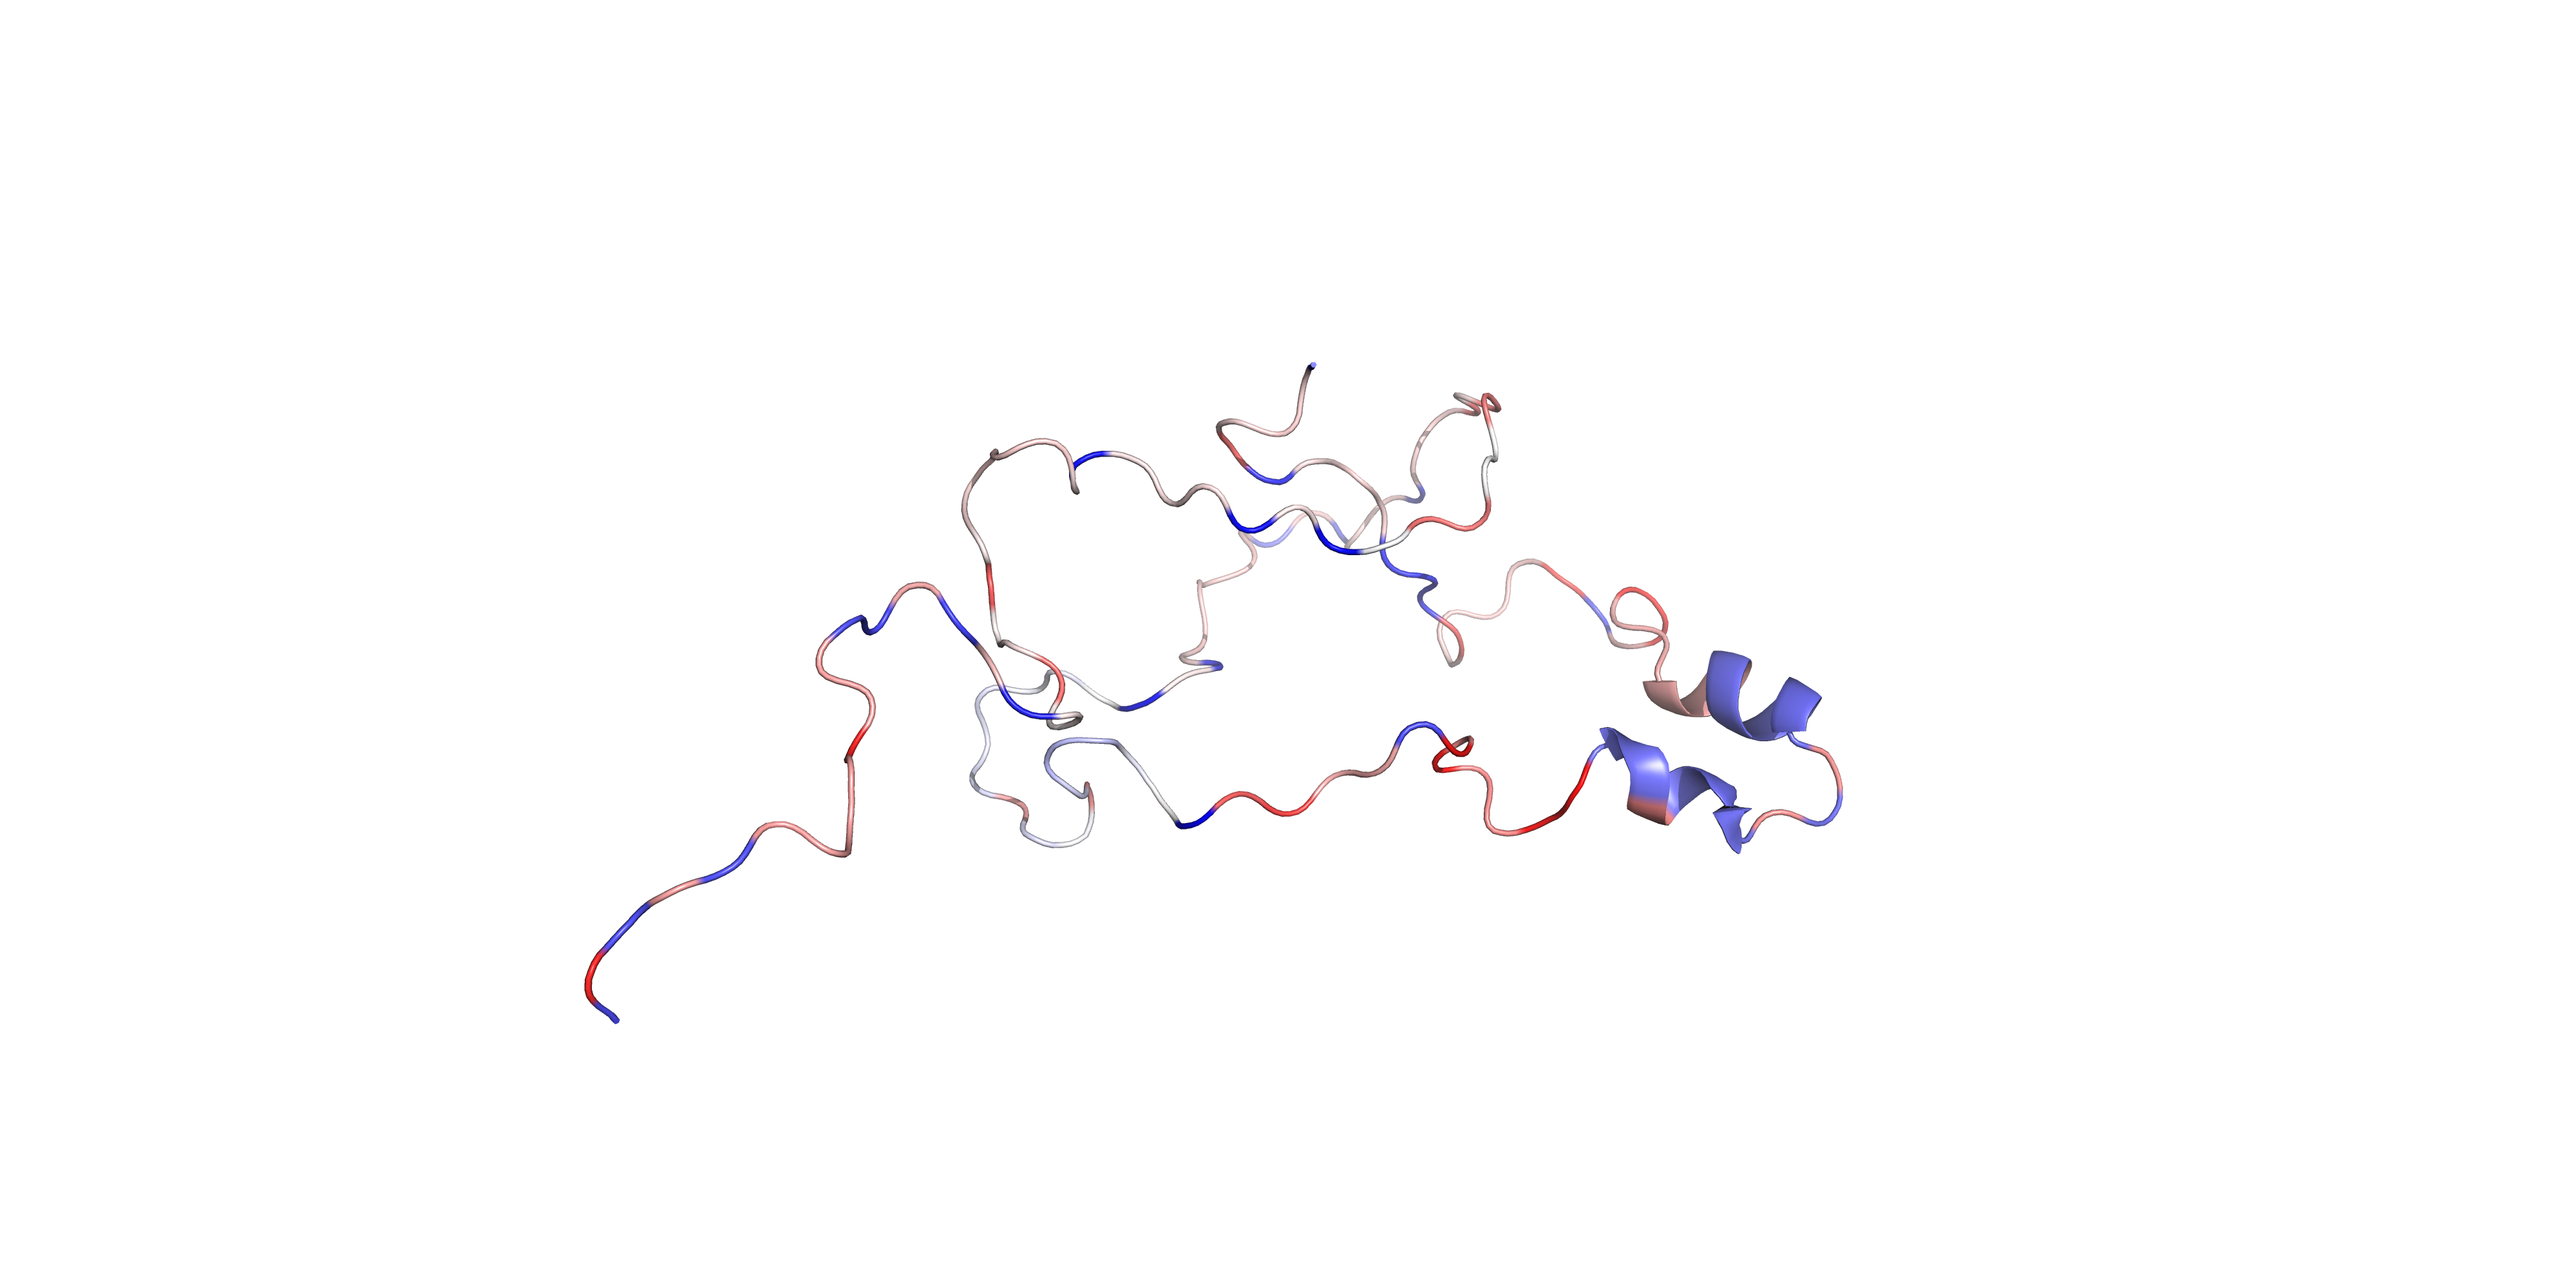
\includegraphics[width=\textwidth]{PED00020e002_pymol.png}
		\caption{Pymol image of model 002.}
		\label{model002}
	\end{minipage}
	\hfill
	\begin{minipage}[b]{0.47\textwidth}
		\centering
		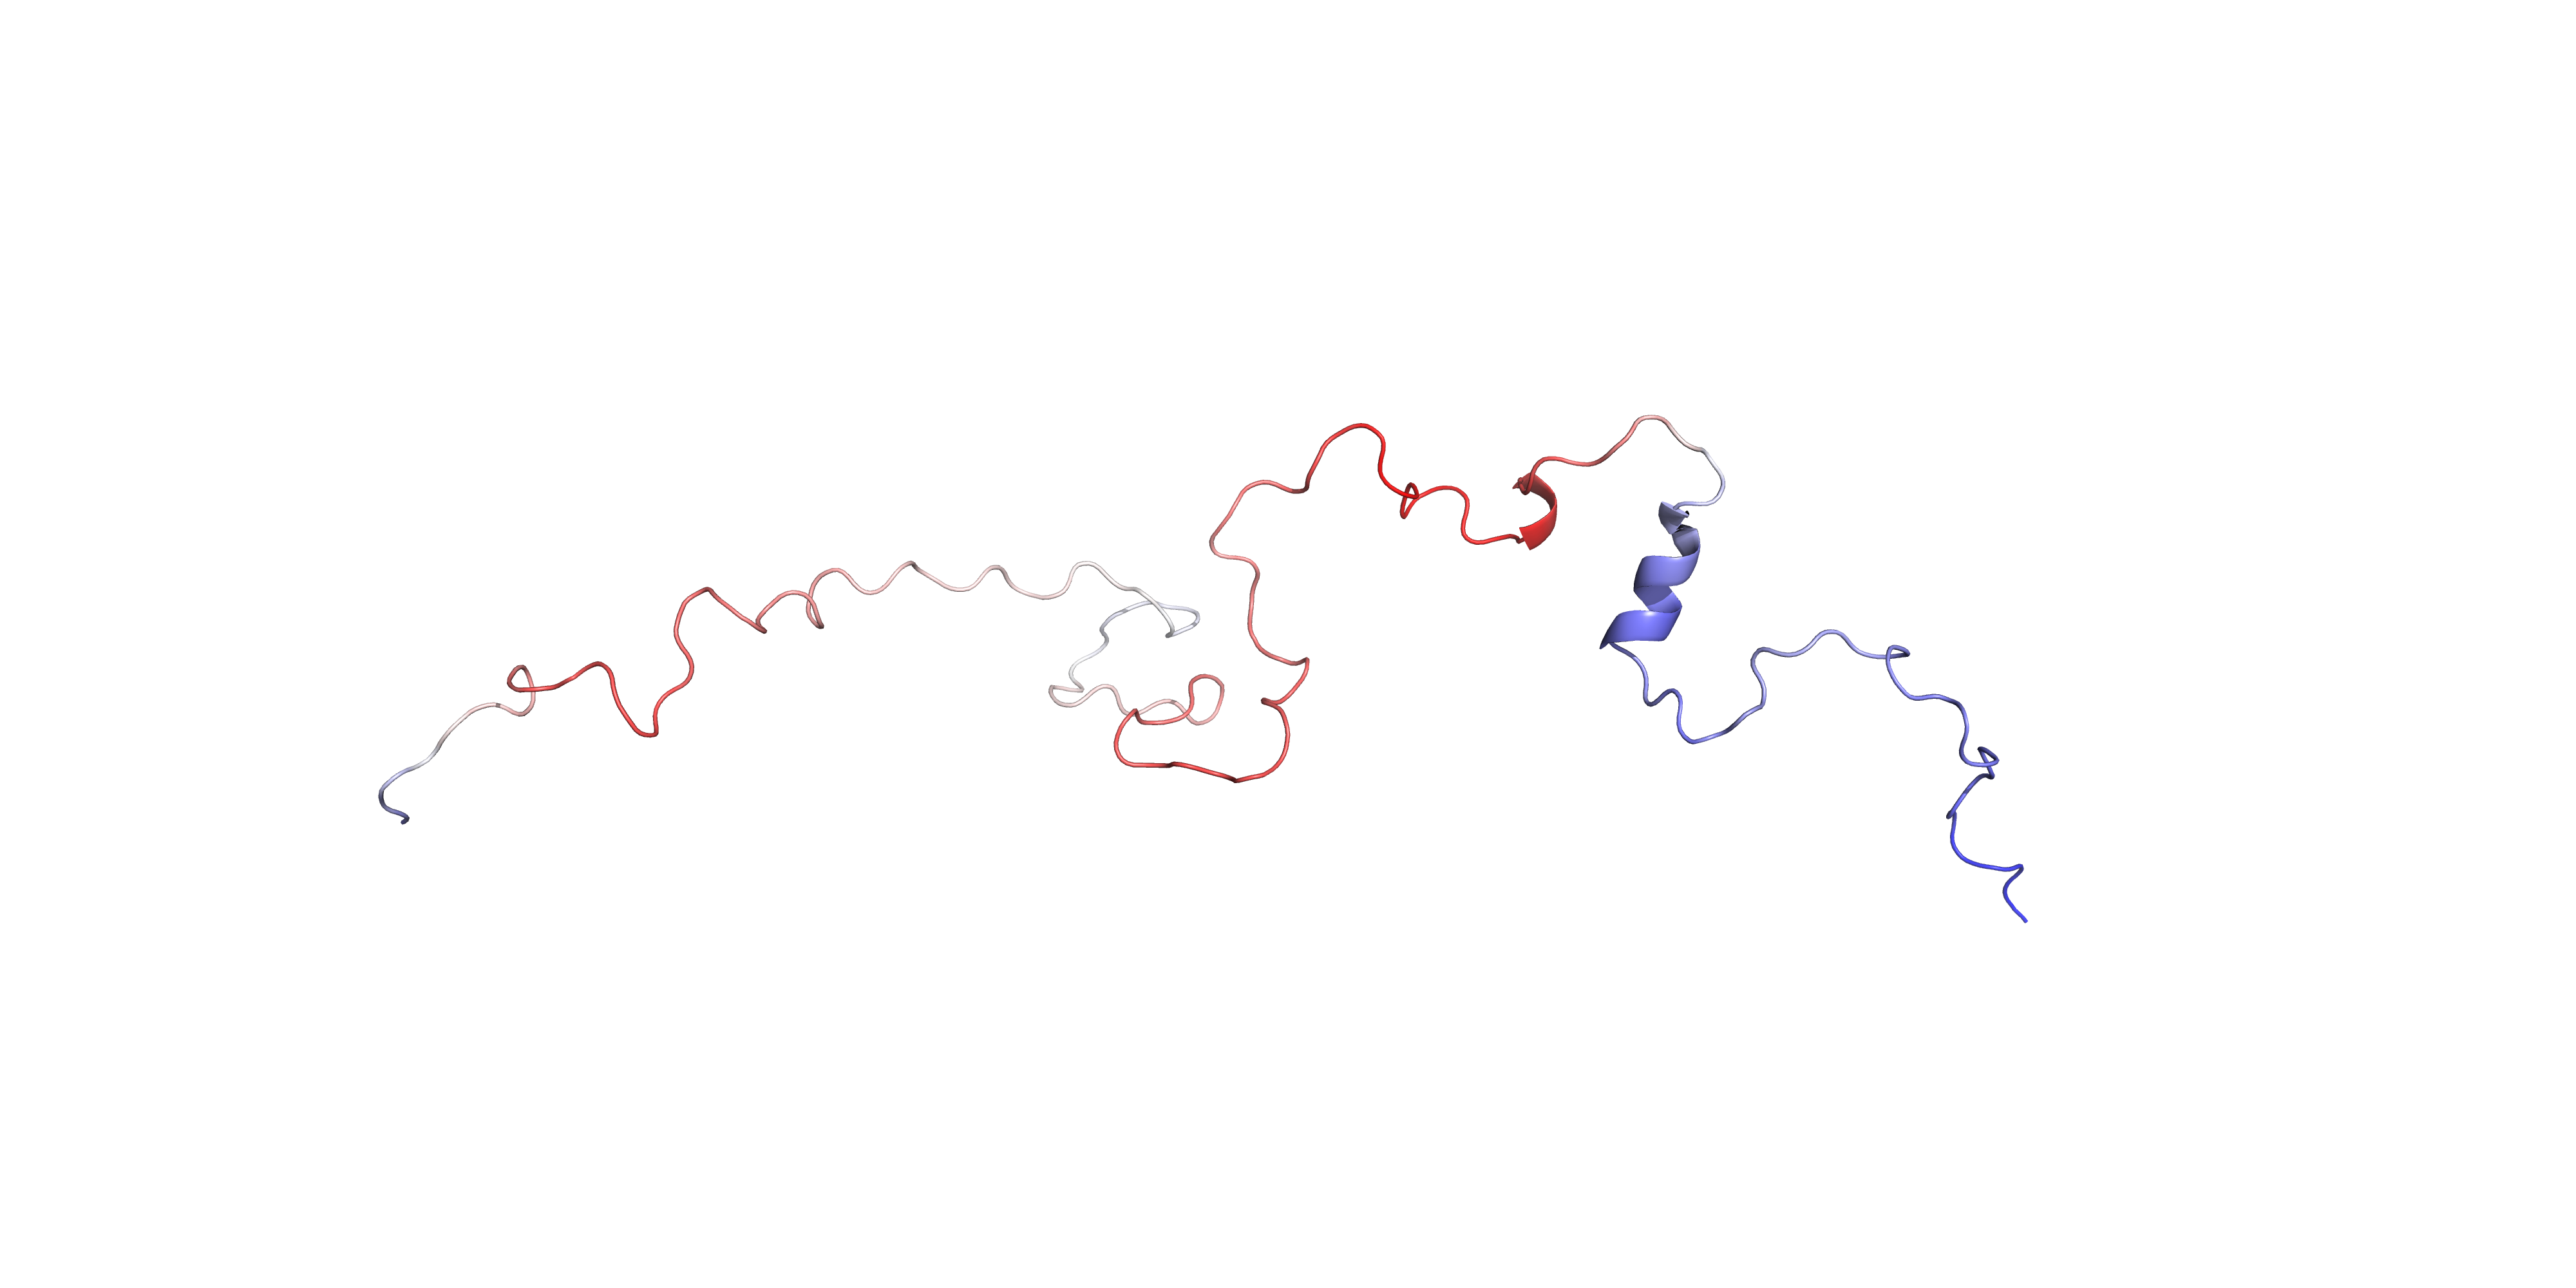
\includegraphics[width=\textwidth]{PED00020e003_pymol.png}
		\caption{Pymol image of model 003.}
		\label{model003}
	\end{minipage}
	\begin{minipage}[b]{0.47\textwidth}
		\centering
		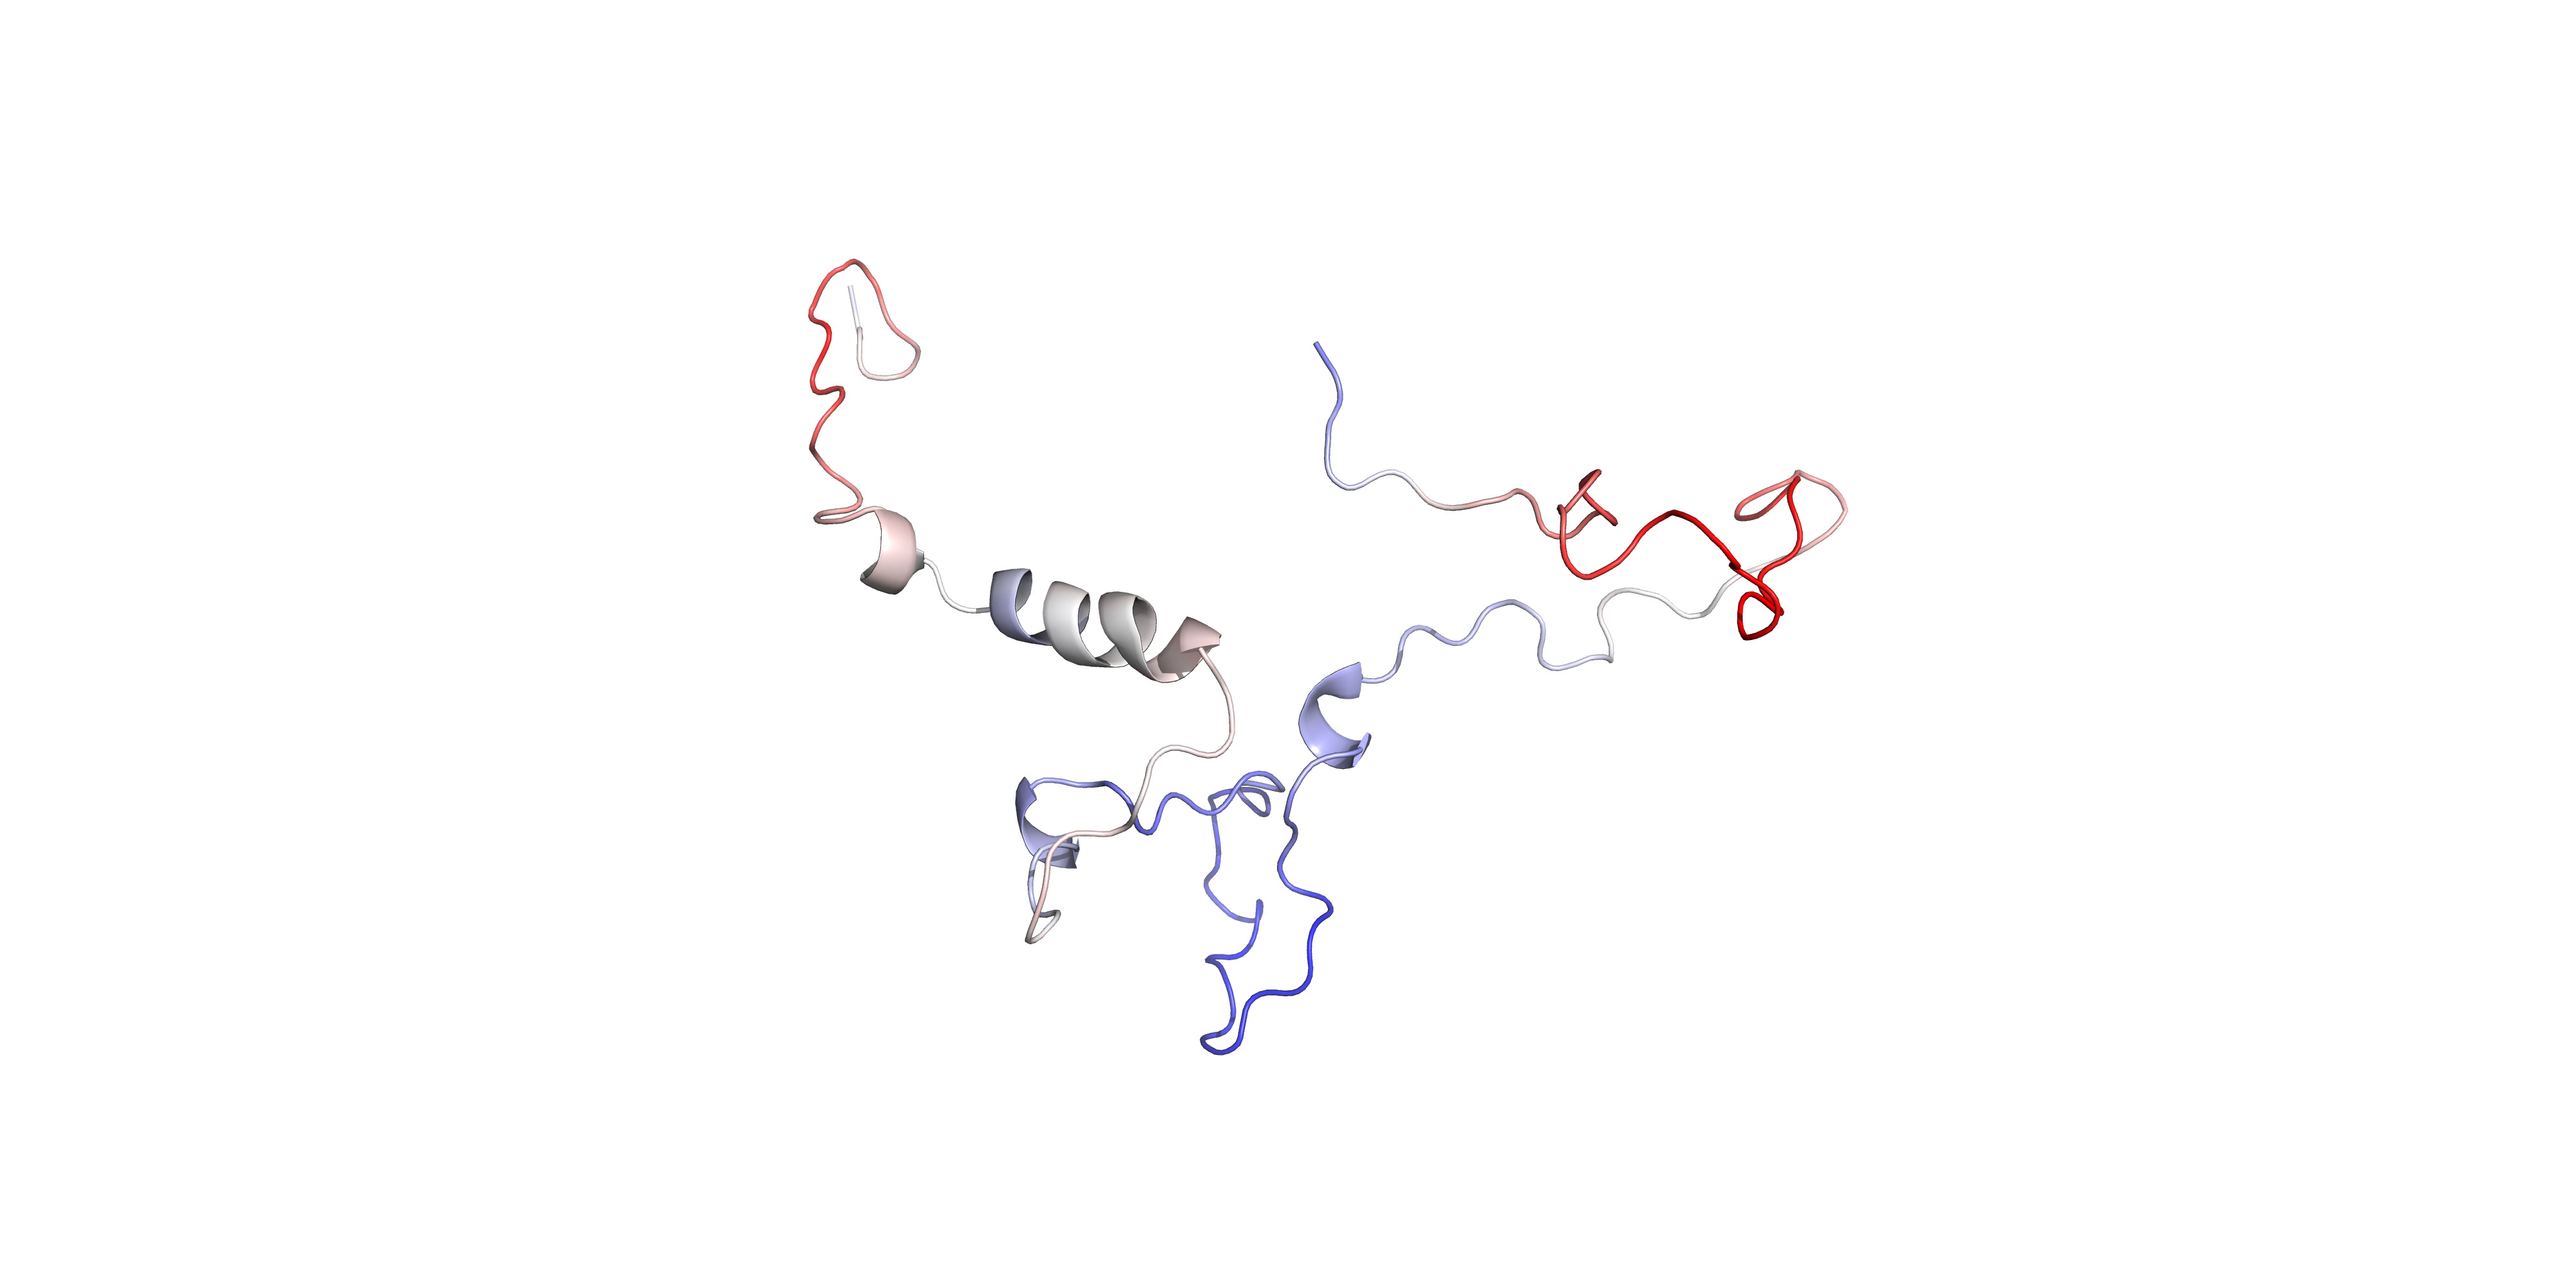
\includegraphics[width=\textwidth]{PED00020e004_pymol.png}
		\caption{Pymol image of model 004.}
		\label{model004}
	\end{minipage}
	\hfill
	\begin{minipage}[b]{0.47\textwidth}
		\centering
		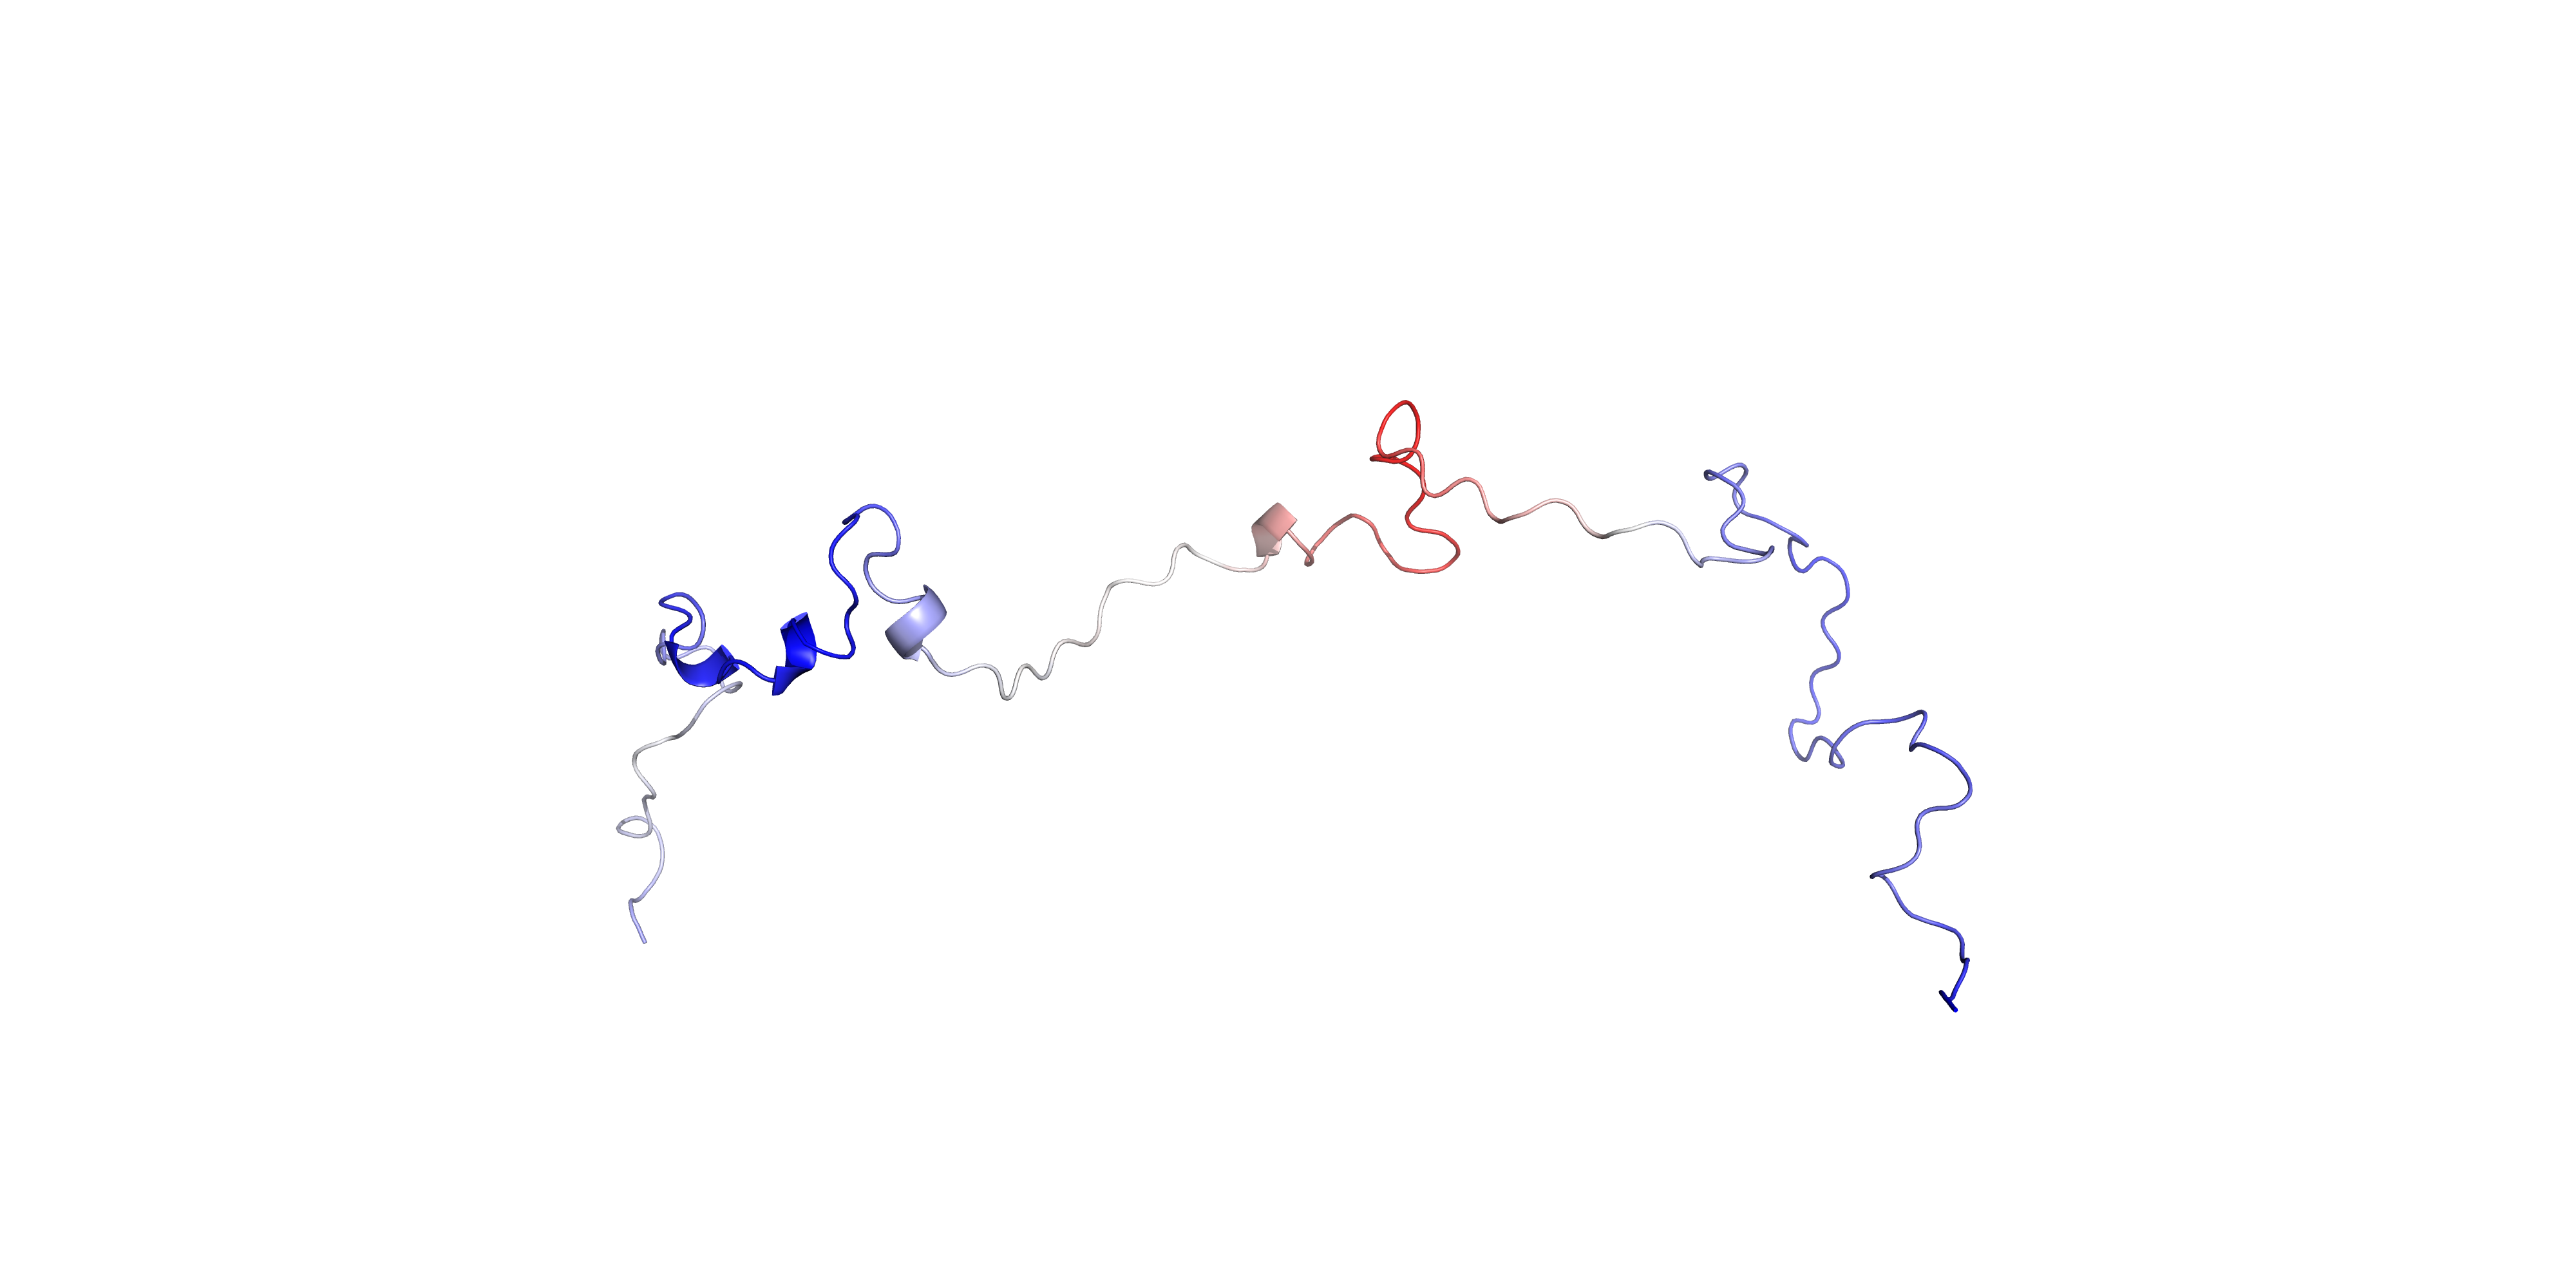
\includegraphics[width=\textwidth]{PED00020e005_pymol.png}
		\caption{Pymol image of model 005.}
		\label{model005}
	\end{minipage}
\end{figure}

Looking at the images you can see that the visualized structures are very disordered and due to the entropic high cost of folding, the well-defined structures (alpha-helicx) are few and mainly in the central regions. In these regions the variability of the representative conformations is less.
